\subsection{Speed analysis}
In this section, average speed and speed distribution for each status are investigated.

The average speed will increase if taxis are occupied. It varies from 25.48 to 27.978 $km/h$ when taxis are occupied, while it ranges from 9.977 to 11.272 $km/h$ when taxis are vacant.



\begin{figure}
\centering
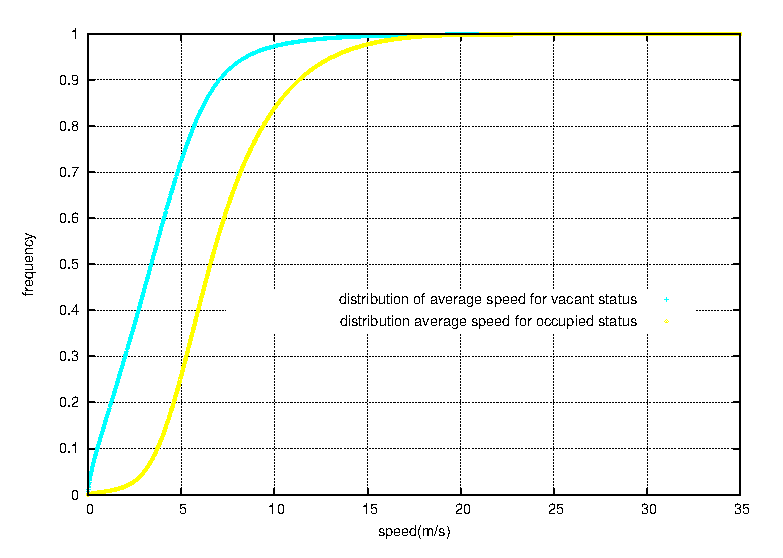
\includegraphics[width=0.4\textwidth]{figures_201103/assumption/speeddis.eps}
\caption{Speed Distribution for vacant and occupied status.}\label{figure_speed_distribution}
\end{figure}

 To further investigate the speed distribution, proportion for every speed section is calculated, in fig.\ref{figure_speed_distribution}. For example, dot(19,0.0245) means $2.45\%$ records fall in the speed range $[19,20)km/h$. Because the proportion for 0km/h reaching up to 20\% is too large compared with the proportion of other speed section, we do not show it in figures.
Fig. \ref{figure_speed_distribution} shows that speed distribution differs for each status. Most speed records are in the speed section $[0,100] km/h$. For vacant status, in the speed section (0,40], it follows a linear distribution. But for occupied status, a peak occurs in the range of $[8,15] km/h$.  Fig. \ref{figure_speed_distribution} also demonstrates that the speed distribution is with strong regularity for each status.


